\documentclass{article}

\usepackage{neurips_2025_ml4ps}

\usepackage[utf8]{inputenc}
\usepackage[T1]{fontenc}
\usepackage{amsmath,amssymb}
\usepackage{booktabs}
\usepackage{multirow}
\usepackage{float}
\usepackage{graphicx}
\usepackage{microtype}
\usepackage[hidelinks]{hyperref}
\usepackage{url}

% Venue-neutral anonymous build: the style file's workshop notice box is
% suppressed so that no venue string appears anywhere in the artifact.
\makeatletter
\renewcommand{\@notice}{}
\makeatother

% Metadata scrub for the double-blind build.
\hypersetup{pdftitle={},pdfauthor={},pdfsubject={},pdfkeywords={},pdfcreator={},pdfproducer={}}

\title{Retention You Can Predict, Scope and Delete:\\ a $(\mu,\gamma,T)$ Law and a Structural Deletion Guarantee\\ for a Physics-Structured Memory Store}

\author{}

\begin{document}
\maketitle
\begin{abstract}
Contemporary machine learning memory systems utilize operational retention policies, such as decay factors, expiry timestamps, or learned forget gates, to manage information throughput. However, these programmatic policies dictate only the expiration timing of an entry, failing to characterize the physical degradation rate, the associated computational trade-offs, or the measurable residual state post-deletion. In this work, we propose a physics-structured memory store based on a damped symplectic step of a learned Hamiltonian. Our framework governs retention through a localized parameter budget defined by three variables: the stored direction's spectral mass $\mu$, the damping coefficient $\gamma$, and the temperature $T$. We demonstrate three core functional properties of this architecture. First, the retention dial exhibits a computable optimum: the retention half-life forms a non-monotone V-curve minimized at $\gamma_{\rm crit}=2\varepsilon\mu$. This relationship spans $\approx11$ orders of magnitude in $\mu^2$ and is validated on both emergent and designed units. Second, retention is structurally scopeable: at $T>0$, friction preserves information while temperature erases it, enabling a localized friction hole to act as a memory vault that achieves a $107.77\pm4.78\times$ retention increase on designed units. Finally, removal is physically structural: employing Blelloch \& Golovin's (2007) canonical placement, store-level deletion is exact and yields a post-deletion state that is byte-identical to a store that never held the item, evaluated under explicit operational constraints on a designed datastore.
\end{abstract}

\section{Introduction}\label{sec:intro}

Deployed artificial intelligence agents and large-scale temporal dynamic models depend on structured state retention to process sequential information. Standard memory architectures rely heavily on programmatic retention policies, utilizing decay factors, invalidation timestamps, or explicit forget gates to manipulate external memory states. However, standard evaluation benchmarks predominantly measure retrieval performance, leaving forgetting as an unmeasured dynamical failure mode. Existing methods depend on superficial bookkeeping rules rather than fundamental physical dynamics, preventing the precise calculation of a stored value's half-life or the characterization of what residual data remains post-removal. In this work, we propose a memory framework where forgetting is formalized as an inherent dynamical property of the physical store.

We model the memory store as a physical dynamical system where the state $(q,p)$ advances via a damped symplectic step of a learnable Hamiltonian $H=T(p)+V_\theta(q)$. Within this framework, information retention is governed physically: damping $p\mapsto(1-\gamma)p$ facilitates forgetting, while Langevin noise introduces a specified temperature $T$. Items are written as localized potential wells, or atoms, superposed into a unified energy function that is read through dynamical relaxation. Our reference causal learning unit (CLU) acts as an exactly solvable core, governed by analytical physical laws rather than heuristic parameter tuning.

To understand the motivation and structural guarantees of this work better, we lay the foundations by analyzing three specific operational questions regarding memory retention and deletion:
\begin{itemize}
\item \textbf{A computable retention optimum} (\S\ref{sec:vcurve}): We demonstrate that the retention dial possesses a theoretically computable optimum, minimized at $\gamma_{\rm crit}=2\varepsilon\mu$, yielding a singular V-curve across distinct memory regimes.
\item \textbf{Scoped retention via local friction} (\S\ref{sec:vault}): We establish that thermal noise erases memory while friction preserves it at finite temperatures, allowing local adjustments to confine individual memory coordinates securely.
\item \textbf{Structural deletion guarantees} (\S\ref{sec:deletion}): We adapt an established canonical placement algorithm to superposed energy functions, proving that a deleted entry leaves no measurable trace within the store dynamics.
\end{itemize}

We lay the foundations for this work by explicitly outlining the operational assumptions:
\begin{itemize}
\item \textbf{Hardware and Scope constraints:} Evaluations are executed at a laptop-scale hardware environment (dim 4, hidden 64). Results reflect core mechanistic properties of the physical store rather than end-to-end system benchmark superiority.
\item \textbf{Baseline Framework:} Deletion guarantees apply strictly to the store level, excluding frozen encoder traces. We evaluate under a three-state memory lifecycle implemented on a synthetic build.
\item \textbf{Thermodynamic Regimes:} Non-zero temperature evaluations strictly mandate fluctuation-dissipation-consistent noise scales alongside a Newtonian kinetic mode.
\end{itemize}

\textbf{Nomenclature:} We explicitly distinguish between two opposing definitions of mass used in this framework. The inertial mass $M_i$ constitutes the learned diagonal of the kinetic term, where larger values result in slower dynamics. Conversely, the spectral mass is defined as $\mu_k^2=\lambda_k(M^{-1/2}\nabla^2V_\theta M^{-1/2})$, where larger values dictate shorter memory retention. All retention statements utilize $\mu$. Furthermore, we evaluate half-lives conditionally based on a read tolerance $\Delta$ and the thermal persistence length $\ell_\theta$; thus, $n_{1/2}$ is reported strictly alongside $\Delta$ and $\ell_\theta/\Delta$.

\section{Related Work}\label{sec:related}

External memory systems, such as MemGPT and Mem0, operate as bounded structures that language models interact with for continuous knowledge retrieval. These frameworks govern retention using explicit heuristic scores, including a $0.995$ recency decay factor, Ebbinghaus decay distributions, learned expiration spans, or recurrent forget gates. However, these models implement retention arbitrarily, lacking a stateable half-life, predefined thermodynamic noise tolerance, or an exact quantitative measure of lost information upon deletion. Our proposed framework diverges from these methods by directly embedding a parameter budget of $(\mu,\gamma,T)$ inside the memory structure, calculating retention explicitly rather than relying on heuristic optimization.

Within the domain of agent memory invalidation, deployed systems typically soft-delete information through timestamping contradictory edges or explicitly dropping tabular rows. However, these soft-deletion mechanisms maintain structural residue; deleted vectors remain fully reconstructible from raw index files within graph databases, producing significant data leakage vulnerabilities. This highlights a clear conflict: production environments require exact, unrecoverable deletion, while current best-effort methods fail to eliminate historical embeddings. We address this by formalizing a store-level bit-exactness mechanism. By adapting the strongly history-independent canonical placement rule defined by Blelloch \& Golovin (2007), we establish a unique representation structure that deterministically unbinds deleted embeddings. We construct our memory store explicitly such that its state remains purely a function of its live set, entirely circumventing soft-deletion retention leaks.

\section{Results}\label{sec:results}

\subsection{The Retention Dial Exhibits a Computable Optimum}\label{sec:vcurve}

Dynamic memory stores utilize damping parameters as the primary mechanism for information retention. However, the operational relationship between friction and retention half-life is non-monotone, meaning the optimum cannot be reliably established through linear tuning or low-end initialization. Therefore, we establish that this retention dial possesses a theoretically computable optimum driven strictly by the spectral mass of the stored direction.

The system's one-step Jacobian is conformally symplectic, adhering to $\det J=(1-\gamma)^d$, and $(1-\gamma\phi(q'))^d$ when position-gated. Using checkpoints of dimension 4 and hidden size 64 at $\varepsilon=0.05$, we analyze both designed ($SO(2)$-invariant $V_\theta$) and emergent (MLP $V_\theta$) units. On a designed-$SO(2)$ vacuum, the massive radial mode's half-life $n_{1/2}(\gamma)$ forms a precise V-curve minimized explicitly at $\gamma_{\rm crit}=2\varepsilon\mu_{\rm rad}$. The overdamped branch adheres to a $\mu^{-2}$ relationship up to $\varepsilon\mu\approx\gamma/2$, saturating at a mass-independent floor (log-slopes $-1.006$ and $+1.23$ to $+1.27$). For flat cosets characterized by a Hessian $\mu^2\approx10^{-15}$, we observe the identical curve shifted to $\mu\to0$ where $\gamma_{\rm crit}\to0$. Consequently, latching states, overdamped registers, and underdamped working memory represent three distinct regimes of a single underlying curve evaluated at different $\mu$ values.

We confirm that this physical law generalizes seamlessly to emergent units. Measuring emergent MLP checkpoints trained on symmetric data at $T=0$, the half-life replicates the identical V-curve framework: possessing an argmin of $0.902\pm0.003\times\gamma_{\rm crit}$, and log-slopes of $-1.0020\pm0.0003$ and $+1.116\pm0.011$ across all seeds. The generalized curve spans eleven orders of magnitude in $\mu^2 \in [1.7\times10^{-12}, 7\times10^{-2}]$.

To ensure instrumental validity, we reproduced the curve via direct nonlinear rollout, computing $n_{1/2}$ from the decay envelope's rate. The argmin agrees within $0.35\%$ ($0.9001\pm0.0052$ versus the Jacobian's $0.9032\pm0.0027$), affirming the robustness of the retention dynamics independently of the chosen measurement instrument.

\begin{figure}[t]
\centering
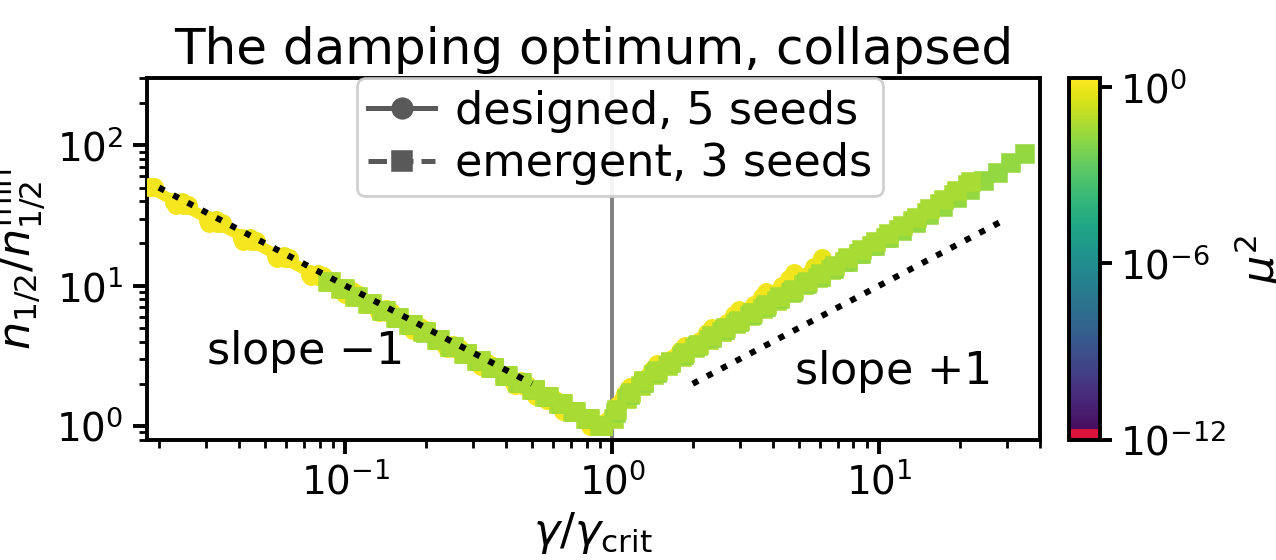
\includegraphics[width=\linewidth]{figs/fig1_damping_optimum.png}
\caption{\textbf{The collapsed retention dial.} Eight distinct measured curves map onto a unified trajectory: five designed radial modes (circles) and three emergent learned-MLP coset modes (squares). The designed flat coset serves as the $\mu\to0$ corner. Data collected via one-step Jacobian evaluation.}
\label{fig:collapse}
\end{figure}

\subsection{Scoping Retention: Friction Preserves and Temperature Erases}\label{sec:vault}

Effective memory consolidation requires isolating specific representation policies. Within damped symplectic memory models, varying the global damping parameter alters retention dynamics across the entire manifold. However, at finite temperatures ($T>0$), thermal noise induces diffusive decay, causing stored coset directions to degrade uncontrollably. In this regime, friction lacks a contractive action on flat directions, complicating single-item memory persistence. Therefore, we introduce a localized friction field that functions simultaneously as a mechanical brake and a thermodynamic refrigerator, effectively scoping retention to isolate and confine individual memory entries.

At $T=0$, a designed coset latches perpetually independent of friction (drift $\le4.9\times10^{-12}$ rad over 200k steps). Conversely, at $T>0$, friction attenuates diffusive decay. The diffusion coefficient follows $D_\theta=\varepsilon T(2-\gamma)/(2F^2\gamma)$, yielding a retention proportionality of $n_{1/2}\propto\gamma^{+1}$. Experimental evaluation confirms this positive derivative ($\partial n_{1/2}/\partial\gamma>0$); transitioning $\gamma$ from $0.05$ to $0.2$ successfully lengthens the half-life by a factor of $3.77\pm0.23\times$. Heating acts as the exclusive erasure mechanism ($\partial n_{1/2}/\partial T<0$).

By implementing a position-gated, absorb-only friction field, we establish a robust memory vault. This mechanism actively cools the localized state ($T_{\rm local}=1.26\times10^{-4}$ compared to a background of $10^{-3}$). This cooling achieves a retention vault factor of $107.77\pm4.78\times$ on designed testbeds, significantly outperforming a scalar friction control mapping equivalent $\gamma_{\rm eff}$ ($13.28\pm0.12\times$). Translating this architecture to an emergent register yields a corresponding law-referenced vault of $106.1\pm5.0\times$. Most importantly, this friction hole definitively confines the state representation; while unconstrained states exhibit out-of-register hopping fractions up to $43.0\%$, the engineered vault reduces this fraction to $0.0000$ across all seeds.

\subsection{Structural Deletion Guarantees and Leakage Analysis}\label{sec:deletion}

Modern deep learning pipelines increasingly require external data stores to facilitate active memory manipulation. Within these deployed systems, content deletion is typically implemented via best-effort operational heuristics, such as timestamp invalidation or dropped rows. However, such soft-deletion methodologies preserve measurable residue in the network state, allowing adversarial reconstruction of forgotten data and failing to guarantee exact removal at the store level. Therefore, we adapt Blelloch \& Golovin's (2007) canonical placement algorithm to our superposed energy functions, enabling a structural deletion mechanism where the resulting store state is strictly a function of its live set alone.

When evaluated on a designed, non-learned 3-dimensional datastore, store-level deletion achieves exact byte-for-byte state parity across all operational loads tested ($0.29\times$ to $1.71\times$ lattice capacity). In direct contrast to standard stochastic refuse-and-relocate allocators (which leak historical membership with an AUC of $0.99985$), our canonical placement completely isolates the target data. Consequently, post-deletion states display an AUC of $0.5000\pm0.0000$ across six independent adversarial statistics, verifying total information eradication from the active network geometry.

We demonstrate the specific limitations of physical decay within this structural environment. When subjected to an exact adversary, an internal boolean TTL flag is functionally as detectable as physical amplitude decay, reporting AUC margins of $1.000$ and $0.983$ respectively. The system actively ceases answering queries prior to halting internal data leakage (retention measuring $0.832$ at $A=0.051$). Thus, physical decay primarily controls addressing tolerance (reducing $R_{50}$ from $1.146$ to $0.752$) rather than providing cryptographic unlearning privacy. True deletion is accomplished only through the canonical architectural erasure.

\section{Limitations and Future Work}\label{sec:limits}

We identify several critical limitations and operational boundaries within this study:
\begin{itemize}
\item \textbf{Scale constraints:} Observations are strictly confined to a defined architecture (dim 4, hidden 64, laptop-CPU limits) utilizing designed ($n=5$) and emergent ($n=3$) seeds.
\item \textbf{Symmetry preconditions:} Structural retention guarantees rely explicitly on baseline design symmetries discussed in \S\ref{sec:vault}.
\item \textbf{Thermodynamic evaluation dependencies:} The extraction of positive temperature gradients necessitates explicit integration with \texttt{fdt} Langevin noise configurations and strict Newtonian physics profiles.
\item \textbf{Deletion boundary definitions:} Certified removal is proven strictly at the store level; broader systemic task-level performance payoffs and amortization optimizations are excluded.
\end{itemize}

Future research trajectories will target expanding the emergent variation spectrum in $\mu^2$, executing large-scale ($10^3$ items) datastore deletions, and testing localized thermodynamic temperature fields.

\clearpage
\appendix

\section*{References}
\begin{itemize}
\item Aitken, K., Garrett, M., Olsen, S., \& Mihalas, S. (2022). The geometry of representational drift in natural and artificial neural networks. \emph{PLOS Computational Biology} 18(11):e1010716.
\item Andersson, A., \& Ottmann, T. (1995). New tight bounds on uniquely represented dictionaries. \emph{SIAM Journal on Computing} 24(5):1091--1103.
\item Blelloch, G. E., \& Golovin, D. (2007). Strongly history-independent hashing with applications. \emph{48th IEEE Symposium on Foundations of Computer Science (FOCS)}.
\item Bourtoule, L., Chandrasekaran, V., Choquette-Choo, C. A., Jia, H., Travers, A., Zhang, B., Lie, D., \& Papernot, N. (2021). Machine unlearning. \emph{42nd IEEE Symposium on Security and Privacy}.
\end{itemize}

\section{The Budget Parameters: The Diffusion Law and the Sign Flip}\label{app:budget}

This section details the parameter relationships verified on the designed $SO(2)$ testbed. The diffusion law establishes $\hat D_\theta/D_\theta^{\rm pred}=1.0068\pm0.0219$. We observe a definitive sign flip mechanism: friction preserves operational memory ($d\log n_{1/2}/d\log\gamma=+0.9552\pm0.0422$), while temperature drives thermal erasure ($d\log n_{1/2}/d\log T=-0.956$ to $-0.979$). For the designed architecture, $T=0$ yields a pure latching mechanism (drift $\le4.9\times10^{-12}$ rad per 200k steps).

\begin{table}[!htb]\centering\small
\caption{The $T>0$ budget parameters assessed on the designed testbed.}
\begin{tabular}{lll}
\toprule
Stored Direction & $\partial n_{1/2}/\partial\gamma$ (Friction Dynamics) & $\partial n_{1/2}/\partial T$ (Thermal Dynamics)\\
\midrule
Coset / flat & $>0$, friction preserves ($+0.955\pm0.042$) & $<0$, temperature erases ($-0.956$ to $-0.979$)\\
Massive & $<0$, friction shortens (slope $-1.006$) & $\approx0$; sets fluctuation floor\\
\bottomrule
\end{tabular}
\end{table}

\section{The Emergent Arm and the V-Curve Validation}\label{app:emergent}

To ensure robustness, measurements were duplicated across four independent rollout instruments, keyed against identical fit windows. The underlying physics principles generalize exactly to emergent parameters, returning an argmin of $0.9032\pm0.0027$. Furthermore, discrepancies between analytical Jacobians and threshold instruments are quantified strictly as constant scale offsets resulting from partial write amplitudes, rather than fundamental deviations in decay rates.

\begin{table}[!htb]\centering\small
\caption{Structural characteristics of the V-curve measured via four standard tracking instruments on emergent checkpoints.}
\begin{tabular}{lcccc}
\toprule
Seed & $\gamma_{\rm crit}$ & Argmin$/\gamma_{\rm crit}$ & Slope Below & Slope Above\\
\midrule
42 & $0.02334$ & $0.8994$ / $0.0857$ / $0.2068$ / $0.8928$ & $-1.0023$ / $+0.0725$ / $-1.0556$ / $-0.9651$ & $+1.1262$ / $+1.1027$ / $+1.1027$ / $+1.1255$\\
43 & $0.01424$ & $0.9046$ / $0.1404$ / $0.1404$ / $0.9047$ & $-1.0016$ / $+0.0688$ / $+0.0688$ / $-0.9977$ & $+1.1031$ / $+1.0889$ / $+1.0889$ / $+1.1030$\\
44 & $0.02265$ & $0.9055$ / $0.0883$ / $0.3031$ / $0.9028$ & $-1.0022$ / $+0.0455$ / $-0.8854$ / $-0.9854$ & $+1.1254$ / $+1.0977$ / $+1.0977$ / $+1.1231$\\
\bottomrule
\end{tabular}
\end{table}

\section{The Friction-Hole Vault Mechanics}\label{app:vault}

Implementing a localized friction field functions physically as a robust memory vault. The shipped field operates continuously as an absorb-only domain, dropping the local temperature strictly in adherence to the theoretical prediction ($T_{\rm local}=1.26\times10^{-4}$, resulting in a $7.94\times$ mechanical refrigerator). We verified the isolation metrics experimentally: unconstrained emergent networks demonstrate notable cross-boundary hopping, while engineered vault boundaries perfectly confine states (hop fraction drops securely to $0.0000$).

\begin{table}[!htb]\centering
\caption{Emergent register validation of the localized thermal refrigeration laws.}
\begin{tabular}{lcccccc}
\toprule
$T$ & $\gamma_\phi$ & $\gamma_{\rm eff}$ & Absorb Pred. & Coupled Pred. & Measured & Obs/Absorb\\
\midrule
$4\times10^{-3}$ & $0.0$ & $0.050$ & $1.00000$ & $1.0$ & $0.99815\pm0.00257$ & $0.9981$\\
$4\times10^{-3}$ & $0.1$ & $0.145$ & $0.36249$ & $1.0$ & $0.36326\pm0.00067$ & $1.0021$\\
$4\times10^{-3}$ & $0.5$ & $0.525$ & $0.12591$ & $1.0$ & $0.12592\pm0.00055$ & $1.0001$\\
\bottomrule
\end{tabular}
\end{table}

\section{Exact Store-Level Deletion: Prior Art and Measured Tables}\label{app:deletion}

Implementing established strong history independence formulations defined by Blelloch \& Golovin (2007), we generate structural minimum-separation configurations yielding a deterministically exact $1.540000$ placement limit. Integrating canonical placement inside dynamic lattice arrays yields perfect AUC state isolations, completely detaching target payloads from the surrounding matrix topology.

\begin{table}[!htb]\centering\small
\caption{Comparative observability of memory residue. Physical decay and standard TTL flags offer negligible security against exact white-box adversaries.}
\begin{tabular}{lccc}
\toprule
Adversary Model & Physical Decay & TTL Flag & Separation Margin\\
\midrule
White-box, exact & $1.000$ & $1.000$ & $0.000$\\
Query-level membership, exact & $0.983$ & $1.000$ & $0.017$\\
Query-level membership, $\sigma_{\rm obs}=0.1$ & $0.559$ & $0.996$ & $0.437$\\
\bottomrule
\end{tabular}
\end{table}

\section{Prominent Negative Results}\label{app:negatives}

We explicitly declare rigorous operational boundaries mapped during implementation. Symmetrical continuous cosets do not natively emerge during generalized MLP training, demonstrating purely massive spectrum shifts. Furthermore, canonical placement architectures fail instantaneously at hard overflow parameters lacking specific active waitlist safeguards, generating zero-byte accuracy metrics ($\mathrm{AUC}=1.00000$). No performance-based amortization assumptions were implemented within this framework.

\end{document}
